\documentclass[fontsize=12pt, paper=a4, headinclude, oneside, pagesize=auto, numbers=noenddot, plainheadsepline, open=right, toc=listof, toc=bibliography]{scrreprt}

% setting line-spacing 
\linespread{1.25}

\setlength{\parskip}{16 pt} 

% Loading Libraries
\usepackage{apacite}
\usepackage[utf8]{inputenc}
\usepackage{eurosym}
\usepackage{amsmath}
\usepackage{graphicx}
\usepackage{pdflscape}
\DeclareUnicodeCharacter{20AC}{\euro}
\usepackage{subfig}
\usepackage{caption}

% changing behaviour of \makechapter manually
\usepackage{etoolbox}
\makeatletter
\patchcmd{\chapter}{\if@openright\cleardoublepage\else\clearpage\fi}{}{}{}
\makeatother


\begin{document}
	\pagestyle{empty}
	
	% Titelseite

	
	\begin{center}
		\begin{Huge}
			Master of Public Policy\\
			\vspace{3mm}
		\end{Huge}{\Large Hertie School of Governance}\\
		
		\vspace{20mm}
		\begin{Huge}
			The Eurosceptic Misfit: Popular Euroscepticism and Electoral Support for Eurosceptic Parties\\
		\end{Huge}
		\vspace{20mm}
		
		\vspace{1cm}
		\today \\
		\vspace{1 cm}
		Malte Berneaud-Kötz \\
		Master of Public Policy\\
		Class of 2016\\
		\vspace{6cm}
		\begin{tabular}{ll}
			{\bf Thesis advisor:} & Prof. Markus Jachtenfuchs\\
		\end{tabular}
		
	\end{center}

\pagebreak

\cleardoublepage
\pagenumbering{gobble}
\tableofcontents
\cleardoublepage

\pagebreak
\pagestyle{plain}
\pagenumbering{arabic}

\chapter{Executive summary}
This master thesis examines the misfit between popular levels of Euroscepticism, defined as any form of opposition to European integration and electoral support for Eurosceptic parties in European Parliament elections. This I call the 'Eurosceptic misfit'. The term 'misfit' was coined by Paul \citeA{Taggart1998}, who suspected that national contextual factors shape the translation of Eurosceptic attitudes into Eurosceptic votes. Despite the advances made in the Euroscepticism literature, this misfit and potential national factors shaping it have received very little scholarly attention. My thesis aims to redeem this shortcoming by conducting the first empirical exploration of the Eurosceptic misfit and national factors shaping it. Combining aggregate national data on Eurosceptic attitudes and aggregated vote shares obtained by Eurosceptic parties in the national European Parliament elections from 1979 to 2009, a data set on the Eurosceptic misfit and national contextual variables is created for the analysis. Visualisations of the Eurosceptic misfit reveal that it is highly volatile, takes wildly different shapes across countries and does not follow clear trends over time. Comparing the Eurosceptic misfit across regions suggests that the Eurosceptic misfit is generally of a smaller magnitude in Central and Eastern Europe. A random effects and a fixed effects model are fitted to the data to explore the effect of general Euroscepticism, instrumental Euroscepticism, party system polarisation, party system fragmentation, EU-membership duration and location in Central/Eastern Europe on the size of the Eurosceptic misfit. The statistical analysis finds that an increase in generally Eurosceptic attitudes in the population increases the size of the Eurosceptic misfit, indicating that vote shares of Eurosceptic parties lag behind the increases of Eurosceptic attitudes. Moreover, there are some tentative indications that higher levels of party system polarisation are associated with narrower Eurosceptic misfits and that Member States in CEE tend to have smaller Eurosceptic misfits when compared to the remaining Member States.

\chapter{Introduction}
In the European Union (EU), we observe a considerable difference between public Euroscepticism expressed in opinion polls and the aggregate vote share Eurosceptic parties receive in the European Parliament (EP) elections. This gap can take different shapes across different Member States. In Germany, there is some popular disapproval of the EU (17\% of respondents to the last Eurobarometer viewed the influence of the EU as 'exclusively negative' in 2015 \cite{Commission2015}), yet German Eurosceptic parties received only around 8\% of the votes in the 2014 EP elections. In France the relationship is the other way around, with relatively moderate popular levels of Euroscepticism, but a huge vote share for the staunchly Eurosceptic Front National.

This misfit between the popular levels of Euroscepticism and the aggregate vote share of Eurosceptic parties was first discussed by Paul Taggart in 1998, when he identified Euroscepticism as a “touchstone of dissent” for mainstream parties \cite[p.~366]{Taggart1998}. He suspected that this misfit must be caused by contextual factors in national party systems. The same 'misfit' between the levels of public Euroscepticism and support for Eurosceptic party has not only been observed in the old EU-15 Member States, but also in the EU-10 countries that joined the EU in 2004 \cite{Taggart2002}. The authors concluded that national parties must play an important part in explaining how Eurosceptic attitudes could potentially shape policy outcomes. Surprisingly, so far no researcher has ever dedicated her time to finding out which national-level variables affect the size of the Eurosceptic misfit, despite the concept being around for close to twenty years. 

The goal of my thesis is to examine this misfit in order to find out whether there are specific factors present on the national level which grow or shrink the Eurosceptic misfit. The Eurosceptic misfit is defined as the share of voters holding Eurosceptic views minus the aggregate vote share Eurosceptic parties received in EP elections. The question that this thesis wants to answer is the following: 
Which national-level properties affect the Eurosceptic misfit observed in the EP elections?

This remainder of the paper will be structured as follows: Chapter 3 gives an introduction to the current state of the Euroscepticism research and the ongoing debates within it. Chapter 4 outlines my theoretical model and hypotheses. Chapter 5 introduces the study data set and describe the operationalisation of variables taken from the hypotheses. Chapter 6 contains both descriptive and inferential statistics carried out on the data. In this section, I will look at whether party system polarisation, party system fragmentation, duration of EU membership or location within Central and Eastern Europe affect the size of the Eurosceptic misfit. In Chapter 7, findings are summarised and avenues for future research discussed. 
 exploratory fashion. 

\chapter{State of the art in Euroscepticism scholarship}

Today, a dynamic research field exists which studies the relationships between public opinion on the EU, party systems at the national level and European party systems. In this triangular relationship, the question of cueing between popular levels discontent with the EU and national party systems received particular attention. Do parties get their cues to be Eurosceptic from citizens, or do party give citizens cues to be more Eurosceptic. Essentially, researchers are asking whether Eurosceptic parties make a country’s population more Eurosceptic or whether Eurosceptic publics bring forth (more) Eurosceptic parties \shortcite<eg.,>{Ray2003,Lubbers2010}. The basic question is: who is cueing whom \cite{Ray2003,DeVries2009}? \shortciteA{DeVries2009} further developed this strand of analysis by also considering the substance of the cues. Another field in the public-party-nexus and Euroscepticism, which is still in its infancy, explores how Eurosceptic parties can shape the agendas of mainstream parties \cite<e.g.,>{Meijers2015}.

\section{Determinants of Eurosceptic attitudes}
A large part of the literature on Euroscepticism deals with the determinants of Eurosceptic attitudes in individuals. The earliest research undertaken has focused exclusively on utilitarian explanations of attitudes towards the EU \cite<e.g.,>{Gabel1998,Gabel1995,Anderson1995}. Scholars in this strand argued that people support or reject the EU because they personally expect to lose or gain from integration. National contexts are the strongest predictors for whether or not a person feels as if they benefited from EU membership, newer studies find\cite{McLaren2007}. Later on, these utilitarian theories have been supplemented by additional identity-based theories, as researchers found that identities can explain large parts of the variation in attitudes towards European integration \cite<e.g.,>{McLaren2002,McLaren2007,Wessels2007}. Another classic theory explaining why people are Eurosceptic relates to cognitive mobilisation \cite{Hooghe2007,McLaren2007,Gabel1998}. This view argues that because voters know very little about the EU and its institutions, and since people fear what they do not know, they come to reject European integration. A fourth explanation for EU-rejection which has been proposed is that since publics are generally poorly informed about the EU, they evaluate it by using their national governments as a proxy. However, empirical evidence on that theory delivers mixed results \cite{McLaren2007}.

\section{Categorisation of Euroscepticism}
As this field of Euroscepticism research developed, the very concept of Euroscepticism has remained very much contested. Therefore, many authors see the need to differentiate it from terms such as 'Europhobia' or 'Eurorealism', as coined by Waclaw Klaus \cite{Kopecky2002}, before conducting any analysis. One of the oldest and broadest definitions is that of Euroscepticism "as an encompassing term" which "expresses the idea of contingent or qualified opposition, as well as incorporating outright and unqualified opposition to the process of European integration" \cite[p.~366]{Taggart1998}. More refined categorisations are based on the notions of 'diffuse' or 'specific' support for political institutions as developed by \citeA{Easton1975} \shortcite<e.g.,>{Gabel1995,Kopecky2002,Boomgaarden2011}. In this context, 'diffuse' is used to describe the ideas an organisation embodies, whereas 'specific' refers to that organisations output. Here, some overlap can be found with Scharpf's notions of input and output legitimacy \cite{Boomgaarden2011}. A further categorisation based on broadly similar distinctions is that between 'hard' and 'soft' Euroscepticism, where 'hard' Eurosceptics reject the integration project outright (similar to the rejection of the 'diffuse' concept of integration). On the other hand, 'soft' Euroscepticism involves contingent or qualified opposition to conferring more power upon the Union \cite{Taggart2004} (similar to the rejection of 'specific' aspects of European integration). Another possible way of categorising is by differentiating between 'political' and 'instrumental' Euroscepticism \cite{Lubbers2005}. In this definition, 'instrumental Euroscepticis' stems from cost-benefit-calculations regarding one's country's membership in the EU. If people think their are paying more into the EU than they are getting back out and they reject integration on these grounds, they will be instrumental Eurosceptics. In contrast, political Eurosceptics refuse to confer more power to the supranational level needed to tackle supranational problems. Individuals can be both instrumental and political Eurosceptics, with them rejecting integration on different grounds. Political Euroscepticism is ordered by the 'national difficulty criterion', meaning that publics are more willing to confer power to the supranational entity to solve problems that are difficult to tackle nationally (such as air quality and environmental protection), but are less willing to confer any powers relating to social protection or redistributive policies \cite{Lubbers2005}.

All this time, categorizing Euroscepticism has proven difficult due to its heterogeneous nature. At a fundamental level lies the demarcation between scholars who study \textit{support} for European integration and those who study the \textit{rejection} of it, both of which can be argued to be very distinct concept in terms of the causal chains on a psychological level \cite{Boomgaarden2011}.

An earlier attempt at categorising was undertaken by \citeA{Kopecky2002}, who created a two-by-two matrix that uses support for European integration as a concept on one axis and support for the EU as it is currently configured on the other. In the face of the EU’s evolving competencies, \shortciteA{Boomgaarden2011} made an argument to move away from the binary for/against-integration conceptualisation of Euroscepticism in the previous literature. Instead, they propose to differentiate between opposition towards different aspects of European integration. Their conceptualisation uses the classic diffuse/specific dimensions, but also distinguishes between the objects of support (the EU regime vs. the community) and between affective and utilitarian motivations to support integration. Throughout these articles, it becomes apparent that authors constantly need to re-define and qualify whether they want to study support of European integration, rejection of European integration, or Euroscepticism as a more abstract concept, with all of these choices having profound impacts on policy and the analyses that follow. 

From the review of the literature, the following picture emerges: while considerable research has been done to examine determinants of Euroscepticism and the direction of cueing between Eurosceptic parties and publics, very few scholars have turned their attention towards the relationship of Eurosceptic attitudes, Eurosceptic votes and how they interact with national party systems. A notable exception is \citeA{Verney2011}, who examined the fit between popular levels of Euroscepticism and electoral support for Eurosceptic parties in Greece and found a surprisingly good fit between the two, contrary to findings in other Member States. The lack of interest in the Eurosceptic misfit is surprising insofar the Euroscepticism literature has made significant advances,yet the Eurosceptic misfit has been neglected almost entirely.

There is some research on how national contexts could affect Eurosceptic votes on an aggregate level, such as \citeA{Taggart2002}. However, their analysis limits itself to comparing patterns of Euroscepticism between Western European Member States and the CEE ones shortly after accession. 

I think that some revision of the topic might be in order. No researcher has tried to find general national-level features of Member States, which allow parties to efficiently leverage Eurosceptic opinion in the public to gain seats in the EP yet. Moreover, Taggart’s and Szczerbiak’s analysis addressed the situation 10 years ago when the EU-10 had just joined, so I expect things to have changed in the meantime. The main point remains that while research into Euroscepticism has diversified significantly in the past 20 years, no-one has yet attempted to conduct an empirical analysis of the Eurosceptic misfit across time and across different EU Member States, leaving this avenue for me to explore. 

\section{Theories on Second-order elections}
A central theoretical assumption underlying this research project is that there is a causal connection between voter's attitudes towards EU integration and their party choice during EP elections. The implicit assumption is made that 'Europe matters' to voters and that it has a measurable impact on their voting behaviour. At first glance this is at odds with the well-established theories on Second-order elections, so despite it not being a part of Euroscepticism literature per se, a discussion of the Second-order election theory and how it affects my research agenda is in order.

The theory was presented in a seminal paper by \citeA{Reif1980}, who argued that European elections could be best understood as a set of simultaneous, national second-order elections, which are essentially fought by national parties in national arenas along national cleavages and using rhetoric that citizens know from national election campaigns. Citizens know that less is at stake in EP elections and consequently behave in a way that is akin to their behaviour in other national second-order elections such as elections to additional chambers of parliament or regional parliaments e.g. German \textit{Landtagswahlen} or British House of Commons by-elections.
The authors derive three core propositions derive from this feature of EP elections: 

1. \textbf{Turnout for EP elections will be lower than for the preceding national election.} The authors argue that this is because voters are aware that "less is at stake" in Second-order elections \cite{Irwin1995}. 

2. \textbf{Big parties will lose vote share} because voters will vote more 'with the heart' than in first-order elections (Reif and Schmitt argued that voters would engage in less strategic voting. However, this view is also contested by \shortciteA{VanDerEijk1996} who argue that voters vote very strategically in elections which happen long after the last national election and which could set 'markers' of party's electoral support prior to the next national election.

3.\textbf{ The result the nationally incumbent party receives depends on the time in the national election cycle the European election is held.} If the election is held right after the national election, the incumbent party should benefit from a 'honeymoon effect'. If it's held in the middle, it will be punished. Towards the end of the cycle, the incumbent party's popularity should recover to normal levels. whether this last relationship holds is not completely certain \shortcite<e.g.,>{VanDerEijk1996,Hix2007}.

The propositions of the original model, which have been slightly refined later on \cite{Reif1984}, have repeatedly received support from various scholars \cite<e.g.,>[p.~2]{Hix2007,Bogdanor1989,Norris1997}, which indicates that voters do not care for European issues in EP elections.
\citeA{Bogdanor1989} has even gone as far deeming it impossible to infer voter's preferences about the EU from their voting behaviour in EP elections. 

It needs to be mentioned, however, that almost all of these studies have tried to make, in one way or another, inferences about the causal mechanisms of individual voting behaviour from aggregate-level data, which makes them prone to committing ecological fallacies \cite{Hobolt2011}. Also, while the Second-order model has received strong support in studies focusing on Western Europe, the relationships predicted seem shakier in the CEE Member States. \citeA{Koepke2006} find that in those countries, voters do not vote to punish incumbents when the European election happens in the middle of the national election cycle, contrary to the findings of the Second-order election model.

Next to the classic view of understanding EP elections as second-order national elections, an alternative viewpoint has emerged arguing that 'Europe matters' \cite{Hix2007}. Proponents of this alternative viewpoint argue that voters have different preferences for different policy arenas and that EP elections are at least partially about European matters. These scholars argue that the defection from governing parties observed at the aggregate level in the Second-order literature must not necessarily be driven by timing of the European election in the national election cycle, but could also be the result of 'European' motivations on the individual level \cite{Hobolt2009a}. However, macro-level models do allow for the disentangling of these two causal mechanisms. As evidence, scholars point to the 'Green tide' experienced during the 1989 EP elections, as well as the establishment of Anti-EU parties in France, the United Kingdom and Sweden. Further evidence suggests that some parts of the electorate vote on European issues. This is probably true for voters of 'Green' parties. Moreover, citizens who are dissatisfied with the speed of European integration have a higher likelihood of defecting from mainstream parties and casting their vote for more radical protest parties closer towards extremes of the traditional left-right continuum. According to \citeA{Irwin1995}, people defect to more radical parties  because all mainstream parties are overwhelmingly pro-integration and there are no alternatives among them which offer a differing vision on the future of the EU, leaving those dissatisfied with the speed of integration two options: abstention or defecting to a radical party. A similar position is shared by \shortciteA{Hobolt2009a}, who find that voters defect because mainstream parties are usually far more pro-European than the median voter. This ties in with earlier research which finds a similar divide between political elites and the broader public \cite{Hooghe2002}. Even \citeA{Hix2007} who accuse proponents of the 'Europe matters' perspective of selectively viewing evidence have to concede that there is empirical evidence that parties with strong positions on the EU tend to do better on EP elections that those having a weaker profile.

In this vein, \citeA{Ferrara2004} find that parties which are not internally divided on EU issues tend to do better in European elections than those who exhibit internal division on the matter of EU integration. The authors theorise that this is because voters want to signal to mainstream party leaderships that they should 'get their act together' and find a coherent position on the matter of EU integration. On a micro-level, the authors suspect that parties which suffer from internal dissent create uncertainty about the leadership's intent and ability to carry out coherent and actionable policy regarding their party's position on integration. This uncertainty causes voters to defect.
Moreover, there is some indication that 'Europe matters', for certain parts of the electorate. Among others, this seems to be also true for voters of Anti-EU parties \cite{Hix2007}.
Also, while \citeA{Hobolt2011} argue that most voters base their votes in the European arena on domestic preferences, voters with addition information about the EU integration tend to base their decisions upon that. Accordingly, there is an argument to be made that for voters who are informed on and have strong opinions about European integration, 'Europe matters'. The crucial point for my thesis is the following: while EP elections are mostly 'national' in nature and electorates 'put the boot in' \shortcite[p.~157]{Marsh2010,VanDerEijk1996} to punish national governments, their decisions are also partially based on European considerations. 

The EP has little power in shaping the future of the EU \cite{Mair2000} and voters are probably aware of the fact that their vote will have little influence on the future of integration. Despite of this, they vote for Eurosceptic parties. This can be understood as a symbolic act through which voters voice their discontent with the European integration project. Through this act, they show that 'Europe matters' to them, which is at odds with the classic viewpoint in the Second-order election. Moreover, this feature allows me to reasonably assume that strongly Eurosceptic citizens would also vote vote for Eurosceptic parties.
Considering that proponents of the second-order model argue that voters behave very strategically, aware of the signals they send to national parties \cite{Boomgaarden2011}, it does not seem far-fetched to assume that voters also use the channel of European elections to send messages about their stance on the EU to national parties.
 Hence considering European elections as being exclusively fought in the national arena, thereby disregarding the European dimension, oversimplifies the factors influencing voter choice and it stands in the way of further investigation of how the two arenas interact. My thesis aims to contribute to the study of this nexus by linking national party systems with voting behaviour in EP elections. 

\chapter{Theoretical model}
As this thesis is primarily concerned with macro-level effects of the properties and structures of the party systems on the transmission of Eurosceptic sentiment into Eurosceptic vote shares, it will use aggregated national data comparing vote shares of Eurosceptic parties with aggregate levels of Eurosceptic attitudes in the respective countries. The difference between the share of the population harbouring Eurosceptic attitudes and the aggregated vote share Eurosceptic parties received in the EP elections, the Eurosceptic misfit, will form the independent variable. 

It is essential to mention that this level of analysis only allows for very coarse explanations of the Eurosceptic misfit. This means that this research can allow for some conclusions on the effect of macro-level variables manifesting in the aggregate outcomes of national-level EP elections. However, it cannot infer to the causal mechanisms that are motivating voter behaviour on the individual level, as this would constitute an ecological fallacy. In order to delve deeper into the causal mechanisms linking together the macro-level properties of party systems and Eurosceptic votes, a multilevel binary model could be a possible approach. However, such a complicated model would exceed the scope of this paper.
Accordingly, the analysis presented in this thesis is of a more exploratory nature on a topic that has received next to no academic investigation so far, trying to establish whether a closer look into the causal mechanisms using individual-level data could be fruitful.

This paper assumes that there is no strong cueing effect between Eurosceptic parties and Eurosceptic attitudes among the public. Existing research points towards the existence of such a relationship \cite{DeVries2009,Lubbers2010}, but there is an ongoing, unresolved debate about the direction of cueing between parties and publics. Unfortunately, if a strong cueing effect of Eurosceptic parties on public attitudes were to exist, this could potentially introduce an element of reverse causation into my model: stronger, more relevant Eurosceptic parties turn voters more Eurosceptic, which in turn empowers those parties to shape discourse more effectively. In this case, my research would suffer from reverse causality, so I assume that cueing from parties to citizens is no significant enough to influence my results. 

\section{Hypotheses}
As there are no direct precedents in terms of theories or hypotheses to build upon, some hypothesis have been borrowed from existing, related Euroscepticism research and studies of national party systems in political science, while other hypotheses are purely exploratory.

\textbf{Hypothesis 1}: I expect that higher levels of popular Euroscepticism are associated with greater Eurosceptic misfits. The assumption is that because Eurosceptic parties are generally outsiders in the party system \cite{Ray2007}, voters are reluctant to vote for them and would rather vote for a party they would also support on the national level. Possibly, voters agree with a mainstream party on most matters except their stance on European integration and thus decide to vote for a pro-integration party, but which is socially accepted and which stands a chance of securing a sufficient share of votes to make a difference, despite their views on integration aligning closer with Eurosceptic parties. Thus, I suspect that a lot of voters vote for mainstream parties begrudgingly, because the Eurosceptic alternative that would echo their position on European integration does not reflect their other preferences.

\textbf{Hypothesis 2} :I suspect that party systems with higher polarisation have a smaller misfit between Euroscepticism and Eurosceptic vote aggregate as compared to party systems where parties cluster around the centre of the ideological left-right continuum or where the extremes of the political continuum are populated by politically insignificant fringe parties. This follows work done by \citeA{Dalton2008}, who argued that increased polarisation in party systems can strengthen the bond between parties and their voters. In general, I assume that more polarised party systems are reflections of underlying polarisations in the electorate and ultimately in the societies that host them. Therefore I expect voters in polarised party systems to be more widely dispersed across the left-right continuum. Taking into account that Eurosceptic parties tend to cluster around the extremes of the party spectrum \cite{Taggart1998,Ray2007}, more voters will have less ideological distance to Eurosceptic parties in polarised party systems as opposed to those where voters cluster around the centre. While political left-right placement can be used as a predictor for Eurosceptic attitudes, \citeA{Hooghe2002} argue that their GAL/TAN dimension is a more accurate predictor of party positions on European integration, so it is reasonable to argue that the same should be true for voters. Just because voters are close to mainstream parties on a left-right dimension, things might look different on a for/against-integration dimension. Transferred to the example of a party system with low polarisation this means that voters could indeed be well-aligned with their preferred mainstream party in terms of left-right orientation, but a significant gap could exist in their preference on European integration and that of the elites of the party elites. Here, I suspect that on average, voters will vote for parties closest to them ideologically on the left-right continuum, but will still remain rather Eurosceptic, creating the 'Eurosceptic gap' that will be analysed in this thesis. Another observed characteristic of European party systems which could contribute to this dynamic is the divide between attitudes towards European integration among party elites and their voters \cite{Hooghe2003}. It is necessary to say that in my case, polarisation serves as a proxy for the underlying distribution of voter preferences, which could lead to more accurate models. Nevertheless, polarisation is by far the best available aggregate-level variable to capture the distribution of voter preferences.

\textbf{Hypothesis 3}: I suspect that the Eurosceptic misfit will be negatively correlated with the number of effective parties in a party system. I assume that a higher number of parties in a system will be an indication of higher fragmentation in the party system, which increases voter choice. This increased choice possibly gives them access to different flavours of Euroscepticism. Voters can vote Eurosceptic without having to compromise as much on other policy positions if a wider range of Eurosceptic parties is present.

\textbf{Hypotehsis 4}: As my last hypothesis, I expect that the Eurosceptic misfit is wider the longer a country has been a member of the EU. I expect this to be the case because of the path dependency associated with EU membership. When countries join the EU, the accession process is often accompanied by a lot of discussions on the ins and outs of membership, but as time passes political elites' preferences converge upon membership, it becomes a given in the national discourse and no mainstream party dares to endorse Eurosceptic positions. As a result, voters with Eurosceptic attitudes have no options among the mainstream parties that would allow them to voice their opposition to the integration process, leading to a greater Eurosceptic misfit. Additionally, including membership duration as a covariate in the statistical model allows me to control for any other affects that are associated with "ageing" in membership, similarly to what is sensible in the study of individuals.

\textbf{Hypothesis 5}: I suspect that there is a significant difference in the Eurosceptic misfit between the CEE Member States, which joined the EU in 2004, and the old Member States which had been part of the Union before. This hypothesis rests on the findings of \citeA{Taggart2002} who examined Euroscepticism in Candidate States before accession. They found higher levels of electoral support for soft Eurosceptical parties overall. In the CEE states, single soft Eurosceptic parties carry more importance in terms of vote share as compared to the 'old' Member States. The latter point indicates that soft-Euroscepticism can be found in more established, 'respected' parties as opposed to being confined to outsiders in the party system, which use their Eurosceptic stance to emphasise their distance from the establishment \cite{Mair2000}. I expect a better fit between the popular levels of Euroscepticism and electoral support for Eurosceptic parties in the new Member States because soft-Eurosceptic parties there are not pariahs of their national party systems.



In order to test any of the hypotheses above, concepts such as Euroscepticism, polarisation, among others, have to be operationalised. This process is outlined in the following chapter. This might seem tedious at first, but is based on the finding that how one treats the data prior to the analysis and how variables are operationalised can potentially have a more profound impact on the final results than the choice of statistical model. In an effort to make this process as transparent as possible, the coding of my variables of interest is explained below. 

\chapter{The study data set}
\section{Data sources}
% Citations for all the data sources are included here
\nocite{EB1979}
\nocite{EB1984}
\nocite{EB1989}
\nocite{EB1994}
\nocite{EB1995}
\nocite{EB1996}
\nocite{EB1999}
\nocite{EB2004}
\nocite{EB2009}
\nocite{EMP}

For this thesis, a panel data set containing national results for the EP election rounds and levels of public Euroscepticism prior to the elections from 1979 to 2009 was built.  Additionally, independent variables were computed for the data set in accordance with my hypotheses. Among these are the number of effective parties, the polarisation index \cite{Dalton2008}, and membership duration.  The data set created is a strongly unbalanced panel which has 110 observations over 7 time periods and 27 unique panel units. It combines data from the following sources:\footnote{Please consult the bibliography for citations of all the data sets used} 

\begin{itemize}
	\item Data on public attitudes towards the EU from Eurobarometer data
	\item Data on party positioning towards European integration from the Euromanifesto Project
	\item Data on outcomes of the national EP elections from the Euromanifesto Project
\end{itemize}

The code used to create my data set and all of the variables involved in the analysis plus extensive documentation can be found on my GitHub repository at \\ https://github.com/mberneaud/EuroscepticMisfitMasterThesis. Upon downloading the necessary data from secondary sources, the source code allows for reproduction of my results. The entire analysis was carried out in R, version 3.2.3 and version 3.2.4. Additional packages used in the analysis are listed in the bibliography. 

\section{Operationalisation}
During operationalisation, the nature of the data available often proved to be a limiting factor between what would be theoretically advisable and what is practically feasible. For example, it would have been very interesting to include data on the 2014 EP elections, but so far no data on the national EP election outcomes for that year have been included in the Euromanifesto Project data set. The section below explains how operationalisation was conducted  despite these constraints, starting with popular Eurosceptic attitudes and a categorisation of Eurosceptic parties, both of which are necessary to calculate my dependent variable: the difference between popular levels of Euroscepticism and electoral support for Eurosceptic parties in EP elections. After that, I will outline the operationalisation of the concepts party system polarisation, effective number of parties and membership duration. 

\subsection{Eurosceptic attitudes of citizens}
For data on Eurosceptic attitudes, I used the Eurobarometer that was conducted in the first half of the year prior to the EP elections, typically in April. I decided to use these over the Barometers directly following the elections, as voters might experience a 'honeymoon phase' in the time after the election, just as is the case with national elections \cite<e.g.,>{Marsh2010,Hix2007,Norris1997}, which could befuddle the results.
An exception are the data for 2004, as the ten CEE Member States had not yet joined the EU when the fieldwork for the Spring-Eurobarometer was carried out. Moreover, the newly joined Member States had their elections mostly in the summer of 2004, so the first Eurobarometer after the accession was used for coding of the Eurosceptic attitudes in 2004. For 2009, the only Eurobarometer before the elections of early June, which also contained the necessary trend variables, was held in January and February already, so there is some unfortunate temporal distance between the recording of the data and the voting process. 

Since the questions and the set-up of the Eurobarometer have changed significantly over the  study period (which covers 25 years after all), only two questions measuring Euroscepticism can be found in all the Eurobarometers selected based on their proximity to the EP elections. The first is a question concerning evaluation of EC/EU membership: "Generally speaking, do you think [OUR COUNTRY]'s membership of the EU is...?" Respondents can choose between four answers which are read out to them in the following order: a "Good thing", "Neither good nor bad", a "Bad thing", or "Don't know". Inappropriate responses differing from the proposed answers are coded as "NA". Because this question does not really fit with any more sophisticated definitions of Euroscepticism beyond the bare-minimum definition of "the idea of contingent or qualified opposition, as well as incorporating outright and unqualified opposition to the process of European integration" \cite[p.~366]{Taggart1998}, I used this variable as a measure of general, all-encompassing attitudes towards Europe and coded all those respondents as 'generally Eurosceptic' who had responded with "A bad thing".
The second question measuring attitudes towards the EC/EU asks respondents whether their country has benefited from EC/EU membership overall: "Taking everything into consideration, would you say that (OUR COUNTRY) has on balance benefited or not from being a member of the the EU/European Community?" Respondents are asked to choose between "Benefited", "Not benefited" and "Don't know" as a list of possible answers. Inappropriate answers are coded "NA". As this question asks respondents to evaluate costs/benefits in a utilitarian fashion, it matches quite well with the notion of "instrumental Euroscepticism" developed by \citeA{Lubbers2005}. Hence, all respondents who answered that their country had not benefited from EC/EU membership are coded as "instrumental Eurosceptics". It is entirely possible that respondents are both generally Eurosceptic and instrumentally Eurosceptic. The two are not mutually exclusive. In fact, 11\% of all respondents in the Eurobarometers included in this study, where both generally and instrumentally Eurosceptic. For better illustration association of the two measures of Eurosceptic attitudes, please consider the cross tabulation below. It shows the shares of Eurosceptic attitudes among all the Eurobarometer respondents that entered the study.

\begin{tabular}{|c|c|c|}
	\hline {\emph{Eurobarometer responses}} & not inst. Eurosceptic & inst. Eurosceptic \\ 
	\hline not gen. Eurosceptic & 65\% & 6\%  \\ 
	\hline generally Eurosceptic & 19\% & 11\% \\ 
	\hline 
\end{tabular} 

Since these two questions are asked right after one another in the battery of questions regarding EU institutions and because both question ask similar things,  one could assume that there is a lot of correlation between the two variables which would make it redundant to examine both of them independently. However, a quick correlation of the the two Euroscepticism variables I created across all Eurobarometers used for the study reveals a Pearson's r of 0.35, which indicates significant correlation, but nothing which would deter me from using both variables. The correlation indicates that respondents are aware of the subtle differences between the questions and that they can differentiate between utilitarian benefit and general attitudes towards EC/EU membership. Because of that, the statistical analysis in the following section of the thesis will include both levels of Euroscepticism as distinct independent variables without much fear of high multicollinearity. 

Because this paper is interested in aggregated levels of Euroscepticism, the individual level data from the Eurobarometers is aggregated into country years, yielding two country-specific shares of Eurosceptic respondents prior to each EP election: One for generally Eurosceptic respondents, one for instrumentally Eurosceptic respondents. On a plus side, this converts the formerly binary Euroscepticism variables into continuous variables making them more suitable for use in Ordinary Least Squares (OLS) regression. However, this comes at the cost of a lot of observations. 

\subsection{Eurosceptic parties}
In determining which parties are Eurosceptic, this paper uses data from the Euromanifesto Project at the \textit{Mannheimer Zentrum für Europ\"{a}ische Sozialforschung}. The data set is created from coding and collecting the party manifestos issued by European parties for the EP elections from 1979 to 2009. Aside from the monumental tasks of coding all the statements available in the manifestos, the researchers also constructed variables summarising party policy stances on a wide range of issues for each election year. These variables include attitudes towards European integration, left-right placement, attitudes towards welfare spending and positioning on a free market/planned economy continuum, among others. This thesis uses the variable mapping the 'pro/contra EU integration' dimension of the parties in the data set to categorise parties as Eurosceptic.
It follows the approach used by \citeA{DeVries2009}, who classify parties as Eurosceptic in relation to the EU-integration-stance of other parties in the same national system. They categorise parties as Eurosceptic if they score more than one standard deviation lower than the national national average on a measure of party stance toward integration. Whereas \citeA{DeVries2009} use data from the 2002 Chapel Hill Expert Survey on party positioning towards the EU, the study in this paper will instead employ data from obtained from coded party manifestos. 

There is an ongoing debate about the validity of using manifesto data to evaluate party stances, as some scholars argue that the data represent the salience of issues rather than the actual party stances, which are hidden underneath the rhetoric of the manifestos \cite{Dalton2008}. While this is a valid concern, this paper ultimately deals with the decisions of voters, whose motivation to vote on an issue stems from the same salience which is captured in party manifestos. Moreover, political parties aim to exploit this salience in order to gain electoral support, so using a classification for Eurosceptic parties based on what they say about European integration vs. their actual stance on integration seems appropriate. 

A different critique of using manifesto data is that there is a difference how parties position themselves on European integration and how they actually act upon it. Another weakness of the manifesto-approach is that European citizens are generally poorly informed on European matters \cite{Hobolt2011}, so it is unlikely that they are aware of what is written inside the party manifestos. They instead rely on news reports and public appearances of party members to base their voting decision on. While a party's behaviour in the political process might not be congruent with the messages in its manifesto, the manifesto serves as an authoritative guideline of the party leadership on the stances to be conveyed during the national election campaigns. Ultimately, it is these messages that are conveyed to voters via the mass media and public appearances of political candidates, so manifesto data serves as valid measure of the party stances on European integration voters are confronted with leading up to the elections. An additional advantage to using manifesto data over expert data (as in the Chapel Hill Expert Survey) is that it does not rate parties on their 'reputation' in mainstream academia, but instead takes the information used in coding party stance straight from the horse's mouth. 

\subsection{The Eurosceptic misfit}
Because the operationalisation as explained above yielded two different measurements for Euroscepticism and deciding between using either one to calculate the misfit is difficult to theoretically justify, an average of the two measures is used in order to compute the Eurosceptic misfit. Accordingly, the Eurosceptic misfit as the dependent variable is calculated as follows: 
\begin{equation}
	ESmisfit_{ct} = (iES + gES) / 2 - \sum_{i=1}^n(VoteShareESParty)_{ict}
\end{equation}


Where \emph{c} is an index identifying the country, observed at time \emph{t}, \emph{iES} denotes instrumentally Eurosceptic attitudes, \emph{gES} denotes generally Eurosceptic attitudes, and \emph{i} is an identifier of the different Eurosceptic parties found in country \emph{c} at time \emph{t}. In the end, this results in a variable which can be either positive or negative. If Eurosceptic sentiment in the population exceeds the vote share obtained by Eurosceptic parties, the Eurosceptic misfit will take on a positive number. In case Eurosceptic vote share exceeds the percentage of Eurosceptic attitudes, the resulting Eurosceptic misfit is negative. Overall, the variable ranges from around -20 to around 42 (see Table ~\ref{fig: summarystatistics}), which shows considerable exploitable variation in the dependent variable. I decided against normalizing the misfit by squaring it similar to a measure of dispersion such as the standard deviation, as a negative and a positive misfit are distinctly different phenomena and I expect them to relate differently to the explanatory variables. Squaring the misfit would assume that low levels of popular Euroscepticism would result in a small misfit, either negative or positive, and that high levels of popular Euroscepticism would result in a larger misfit, regardless of direction. On the contrary, I expect positive and negative misfits to be distinctly different phenomena, so I decided to keep them as they were generated by the computation.

\subsection{Party system polarisation}
For the purposes of this paper, polarisation in the party system is measured using an indicator developed by \citeA{Dalton2008}. His inspiration came from the fact that most scholars use the number of parties in a party system or the vote share of the biggest party as a measure of polarisation within the system. However, this does not account for the differing electoral strengths and the relative positions of parties on the left-right continuum. For example, if many smaller parties exist but are clustered around the mean party-position on the continuum, taking the number of parties would leave us to believe that the system is polarised, but it really is not. The same goes for systems where two big parties exist on different ends of the continuum, where the number of parties as an indicator for polarisation would lead us to falsely believe that the system is not polarised, while in reality strong polarisation exists. Dalton's computation of the polarisation indicator for the party system is done with the following equation,
\begin{equation}
PI=\sqrt{\sum{p_i * ((L/R Score_i - Mean L/R Score) / 5)^2}}
\end{equation}

where \emph{i} denotes the different parties in the system, \emph{p} denotes the vote share in percent a party received during the last election, \emph{L/RScore} denotes the position of the party on a 10-point left-right scale and \emph{MeanL/RScore} denotes the mean of the left-right scores of all parties present in the system.  

The resulting Polarisation Indicator (PI) ranges from 0 to 10 and is comparable to the standard deviation in that it measures dispersion of parties on the left-right continuum. When all parties cluster on the mean L/R position it is 0, when all parties are split between the two extremes, it is 10. 

As the data set used in this thesis also contains a ten point scale measuring left-right placement of parties similar to that used by Dalton, the equation was applied without transformation to the study data set. I created Polarisation Indices for the distinct national party systems during each election round, which results in a total of 111 different indices. Differing from Dalton's approach, the party positioning measure used in my analysis is not computed from voter perceptions of party positions, as such data was not available for all points in time covered by the analysis. Instead, the left-right scale I used was created by the coders of the Euromanifesto data. This is a compromise given the limited availability of data on voter's perception of party stances. Nevertheless, future analyses of the Eurosceptic misfit could gain from looking at voter perceptions of parties instead of expert ratings, as this would be closer to the causal process captured by the other explanatory variables, which is voter attitudes towards the EU and vote share of Eurosceptic parties.

\subsection{Effective number of parties}
Another variable of interest is the effective number of parties. The effective number of parties is a measurement developed by \citeA{Laakso1979} as a measure of fragmentation within party systems which accounts for the size of parties. It does so by excluding parties which participated in the national elections, but which did not win any seats and by controlling for the share received by each individual party. The computation is carried out using this formula:
\begin{equation}
 N = \frac{1}{\sum_{i=1}^n p_i^2}
\end{equation}


Where \emph{N} denotes the effective number of parties in the party system, \emph{i} denotes the individual parties within the system and \emph{p} denotes the vote share obtained as a fraction of 1 (e.g. 23\% vote share translates to a fraction of 0.23). The resulting index \emph{N} can range from 1 to infinity.

This computation makes the index much more representative when comparing party systems across countries as it can control for the inflation of party numbers in countries with lots of very small special-interest parties without electoral relevance. However, one trade-off is that the index over-states the number of effective parties in systems where lots of small parties exist which also obtained seats in the parliament. This leads to very small \emph{p}'s, which ,after squaring and summing, result in a tiny number in the denominator of the formula. As a result, the index number will come out bigger than then absolute number of parties in the system. This is mentioned here because similar results are observed for three observations in the data set, where the index exceeds 20 parties. The number of effective parties represents an \emph{index} of the number of parties rather than an \emph{absolute} value. This is important when following along with the interpretation of statistical results. In one of the observations of the data set, the computation of the number of effective parties actually computed to "infinity", which meant that this observation had to be dropped(compare ~\ref{fig: summarystatistics}). This also restricts all statistical the models to 110 observations in total due to list-wise deletion of observations. 

\subsection{Membership duration}
I calculated the membership duration in years as the difference between the year of the respective EP election and the year a Member State joined the EU.
As with the other variables, summary statistics can be found in the table below. 


% Table created by stargazer v.5.2 by Marek Hlavac, Harvard University. E-mail: hlavac at fas.harvard.edu
% Date and time: Di, Mai 03, 2016 - 20:11:54
\begin{table}[!htbp] \centering 
  \caption{Summary Statistics} 
  \label{fig: summarystatistics} 
\begin{tabular}{@{\extracolsep{5pt}}lccccc} 
\\[-1.8ex]\hline 
\hline \\[-1.8ex] 
Statistic & \multicolumn{1}{c}{N} & \multicolumn{1}{c}{Mean} & \multicolumn{1}{c}{St. Dev.} & \multicolumn{1}{c}{Min} & \multicolumn{1}{c}{Max} \\ 
\hline \\[-1.8ex] 
Eurosceptic Misfit & 111 & 12.831 & 13.365 & $-$20.280 & 42.109 \\ 
General Euroscepticism & 111 & 15.650 & 10.378 & 1.646 & 45.864 \\ 
Instrumental Euroscepticism & 111 & 29.678 & 17.864 & 0.000 & 74.451 \\ 
Polarisation Index & 111 & 3.683 & 1.358 & 0.000 & 6.496 \\ 
Effective Number of Parties & 110 & 5.883 & 5.578 & 1.540 & 42.667 \\ 
Membership Duration & 111 & 22.820 & 18.098 & 0 & 57 \\ 
\hline \\[-1.8ex] 
\end{tabular} 
\end{table} 


\chapter{Statistical Analysis}

\section{Statistical models}
As mentioned earlier, no former investigation of the Eurosceptic misfit exists, meaning that there are no academic papers which could provide guidance or inspiration for the statistical model employed to study the misfit.
Considering the structure of the data set, which contains observations across countries and across time, the analytical approach most feasible for data structured this way is using panel methods. Most of these methods are adopted from econometrics, as econometricians often deal with country-level data with a relatively high number of observational units in combination with short timespans.

There are three methods which are theoretically feasible considering the data observed. One way is (1) treating the data as pooled cross-section and running a linear model on the data with year dummy variables for all but one year. While this allows me to model time-trends by allowing varying intercepts for all years, it exploits the variation between Member States, which does not take into consideration unobserved heterogeneity which is present between the panel units (the Member States). An alternative to that is to (2) estimate a fixed effects model (also called the "within estimation"). This entails time-demeaning the data and performing a linear regression on the data, which allows observation of changes "within" the observational units over time.
The big strength of this approach is that the transformation removes all time-invariant variables from the data, also sweeping away any unobserved heterogeneity which most certainly exist between the different countries and which cannot be captured in the model (e.g. culture of political debate, propensity towards protest voting). Moreover, estimating a fixed effects model is essentially like including a dummy variable for each country in the data set. It captures unattributed country-specific variation like a country-dummy would and thus allows the model to account for this country-specific variation. This is especially useful because our observational units are not drawn from a random sample, which influences the distributions of the explanatory variables.  However, this comes a the cost of efficiency when compared to the pooled OLS model, making it less likely to detect statistically significant relationships. A middle ground between the two approaches is (3) running a random effects model, which entails quasi-demeaning using a Generalized Least Squares transformation and then running a linear model on the resulting data. This approach has two advantages: First, it is more efficient than the fixed effects model. Second, it allows for the inclusion of time-invariant explanatory variables without the need of introducing them in interaction terms. The main drawback of a random effects model is that it requires the assumption that any of the unobserved heterogeneity is uncorrelated with all of the explanatory variables in the model at all times. This is a strong assumption and difficult to argue given the limited number of variables in the data set used.
Because it is difficult to predict a-priori how each of the models will fare in practice, I will model the three different models outlined above first, then compare and contrast the results as far as possible.


The first model calculated was a pooled cross-section including year dummies using the following formula, where \emph{u} is the error term. Please note that the terms "Eurosceptic" and "Euroscepticism" have been shortened in all formulas to "\emph{EUS}" to make them shorter and easier to read. 
\begin{equation}
\begin{split}
EUS.Misfit = \beta_0 + \beta_1 General.EUS + \beta_2 Instrumental.EUS + \\
\beta_3 Polarisation.Index + \beta_4 Effective.Number.of.Parties + \\
\beta_5 Membership.Duration + \beta_6 CEE.dummy + \\
\beta_7 1984.dummy + ... + \beta_k 2009.dummy + u
\end{split}
\end{equation}

The second model is a fixed effects model which takes the following form after time-demeaning the data. The double dots indicate that the variables have been time-demeaned. In this model, $\ddot{u}_{it}$ denotes the time-variant error for panel unit \emph{i} at time \emph{t}. Note that the dummy variable for the CEE countries is swept away during the transformation, as it is a time-invariant variable.
\begin{equation}
\begin{split}
\ddot{EUS.Misfit}_{it} = \beta_1 \ddot{General.EUS}_{it} + \beta_2 \ddot{Instrumental.EUS}_{it} + \\
\beta_3 \ddot{Polarisation.Index}_{it} + \beta_4 \ddot{Effective.Number.of.Parties}_{it} + \\
\beta_5 \ddot{Membership.Duration}_{it} + \ddot{u}_{it}
\end{split} 
\end{equation}

The third model which was estimated is a random effects model using the following formula. The tilde denotes that the data has been quasi-demeaned and $v_{it}$ denotes the quasi-demeaned composite error term. This error term contains both the time-invariant error individual to the panel unit $a_{i}$ and the time-variant error $u_{it}$ which changes with \emph{t}. 
\begin{equation}
\begin{split}
\tilde{EUS.Misfit_{it}} = \tilde{\beta_0} + \beta_1 \tilde{General.EUS_{it}} + \beta_2 \tilde{Instrumental.EUS_{it}} + \\
\beta_3 \tilde{Polarisation.Index_{it}} + \beta_4 \tilde{Effective.Number.of.Parties_{it}} + \\
\beta_5 \tilde{Membership.Duration_{it}} + \beta_6 \tilde{CEE.dummy_{it}} + \tilde{v_{it}}
\end{split}
\end{equation}


\section{Descriptive statistics: the Eurosceptic misfit over time}
Prior to estimating any statistical models on the available data, it makes sense to get a better understanding of the misfit. To this end I examine three aspects of the Eurosceptic misfit: how its mean across Member States evolved over time, which patterns it exhibits in the original 6 EC/EU member states (EU-6) and whether there are regional trends in the misfit. 

\begin{figure}
\centering
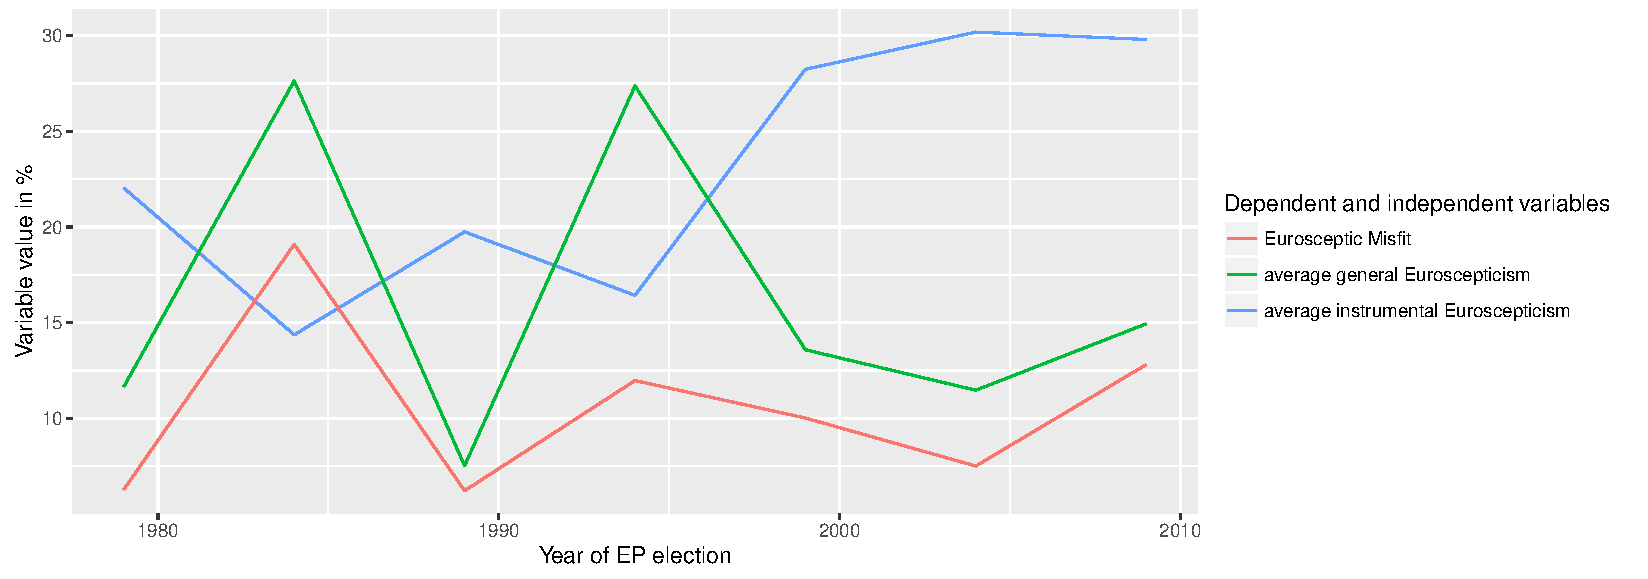
\includegraphics[width=1\linewidth]{../../Analysis/Graphs/DP_and_IVs_over_time}
\caption{EU-average Eurosceptic Misfit 1979 to 2009}
\label{fig:DP_and_IVs_over_time}
\end{figure}

Figure ~\ref{fig:DP_and_IVs_over_time} graphs the mean Eurosceptic misfit, mean average Eurosceptic attitudes (average from general and instrumental Euroscepticism) and mean Eurosceptic party aggregate vote share across all Member States from 1979 to 2009. We observe a Eurosceptic misfit which stayed relatively constant over time, with the exception of the 1984 elections, where high Euroscepticism was paired with very poor electoral performance of Eurosceptic parties, resulted in an unusually large misfit. An interesting observation which can be derived from the figure is a trend of a slightly increasing Eurosceptic vote share from 1984 to 2004, which accompanied the erosion of the "permissive consensus" \cite{Marks2009}. Over the same time period, average popular Euroscepticism increased slightly alongside it. The interesting point here is that on an aggregate-level, the misfit remains relatively stable.


\begin{figure}
	\caption{The Eurosceptic misfit in the original EU-6 over time \\ \emph{Please note that the colour-coding differs from the previous figure}}
	\label{fig: Misfit EU-6}
\begin{tabular}{cc}
	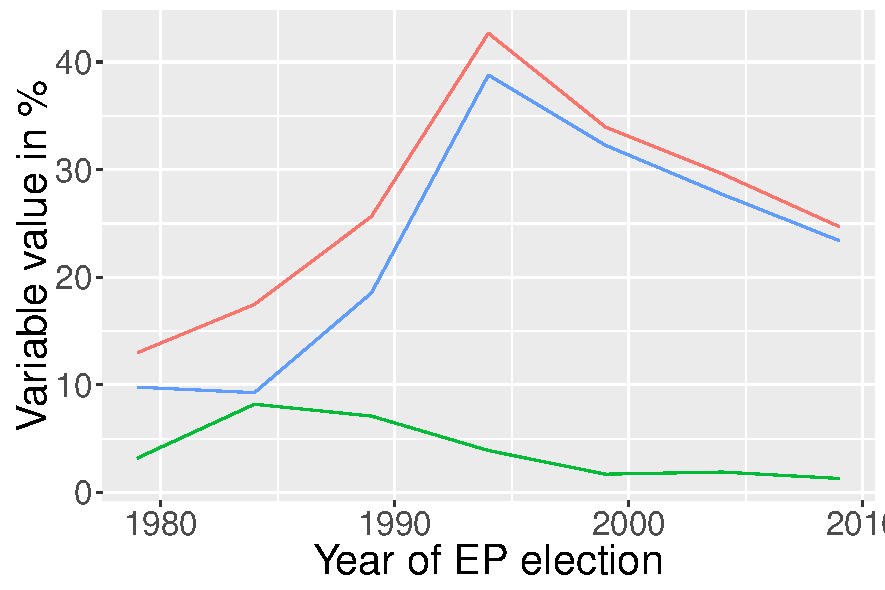
\includegraphics[width=65mm]{../../Analysis/Graphs/DE} & 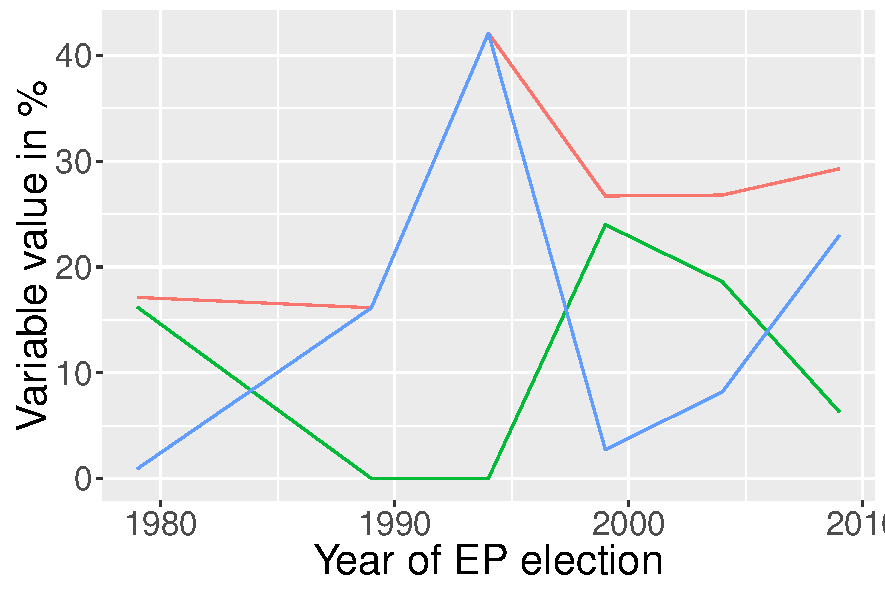
\includegraphics[width=65mm]{../../Analysis/Graphs/FR} \\
	(a) Germany & (b) France \\[8pt]
	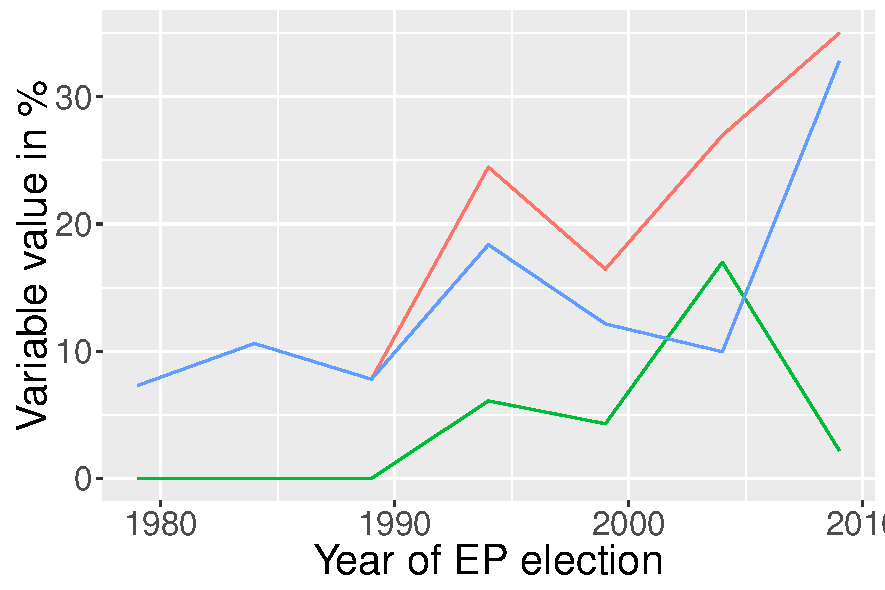
\includegraphics[width=65mm]{../../Analysis/Graphs/IT} & 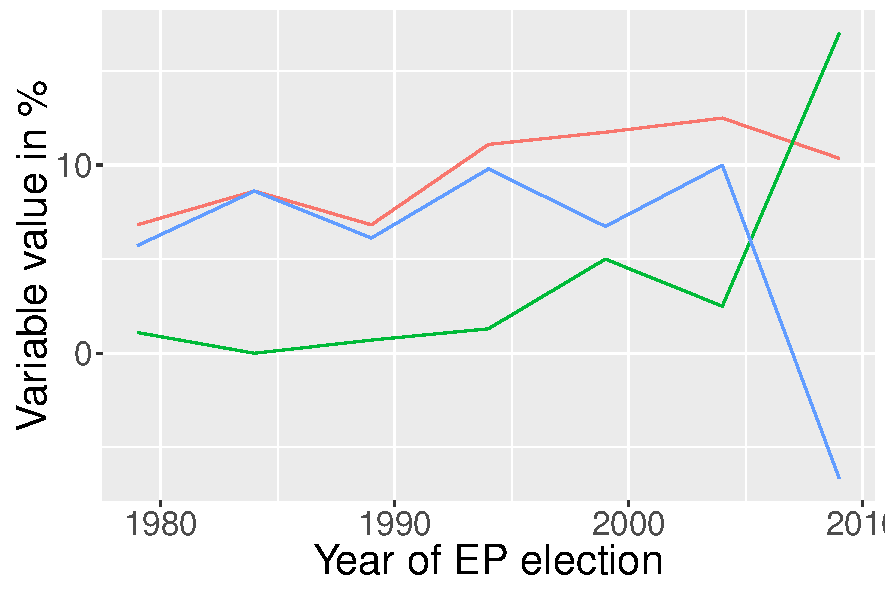
\includegraphics[width=65mm]{../../Analysis/Graphs/NL}	\\
	(c) Italy & (d) The Netherlands \\[8pt]
	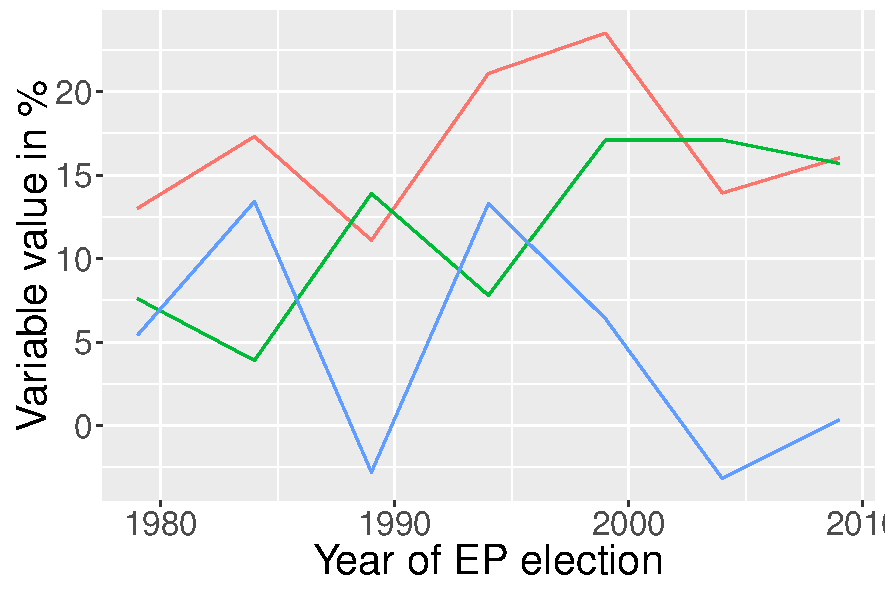
\includegraphics[width=65mm]{../../Analysis/Graphs/BE} & 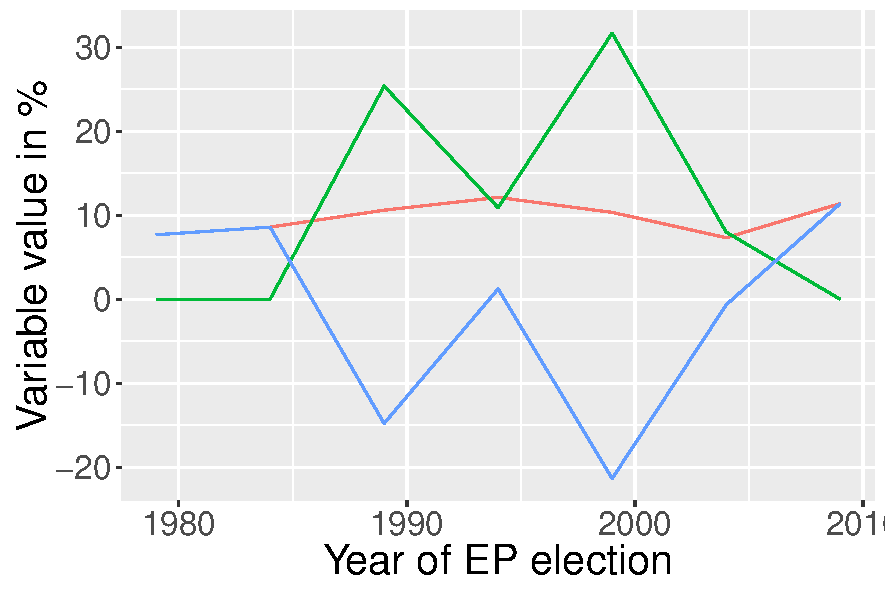
\includegraphics[width=65mm]{../../Analysis/Graphs/LU}	\\
	(e) Belgium & (f) Luxembourg \\[8pt]
\end{tabular}
\caption*{Red: popular Euroscepticism \\ Green: Eurosceptic misfit \\ Blue: Eurosceptic vote share}
\end{figure}
\pagebreak

Looking at the development of Euroscepticism within the original six Member States in Figure ~\ref{fig: Misfit EU-6}, France, Luxembourg and Italy exhibit particularly interesting patterns. In France, the Eurosceptic misfit is very unstable. Here, increasing levels of Euroscepticism are matched with very high vote shares for Eurosceptic parties in some years, but very low Eurosceptic vote shares in others, which results in a wildly fluctuating misfit. Luxembourg's misfit follows a similar pattern, with the striking difference that in Luxembourg, popular Euroscepticism is rather low but vote share for Eurosceptic parties is very high during certain elections, which resulted in huge negative misfits in the 1989 and 2004 elections. Italy is an interesting case because Euroscepticism there follows a clear upward trend beginning in the late 1980s, which only very weakly reflected in the vote shares of Eurosceptic parties until 2004, when they experienced a large spike in support, but which collapsed again during the 2009 elections. The Netherlands display another interesting pattern. Here, we observe rather stable observations for all three variables until 2009, when Eurosceptic parties swept the polls, Eurosceptic party vote share caught up with popular attitudes, shrinking the misfit greatly. This could indicate some very strong protest voting for some Eurosceptic parties, or former mainstream parties having become more Eurosceptic in the meantime, which caused them to be included in the aggregate Eurosceptic vote share. 

\begin{figure}
	\caption{The average Eurosceptic misfit across regions}
	\label{fig: Misfit Regions}
\begin{tabular}{cc}
	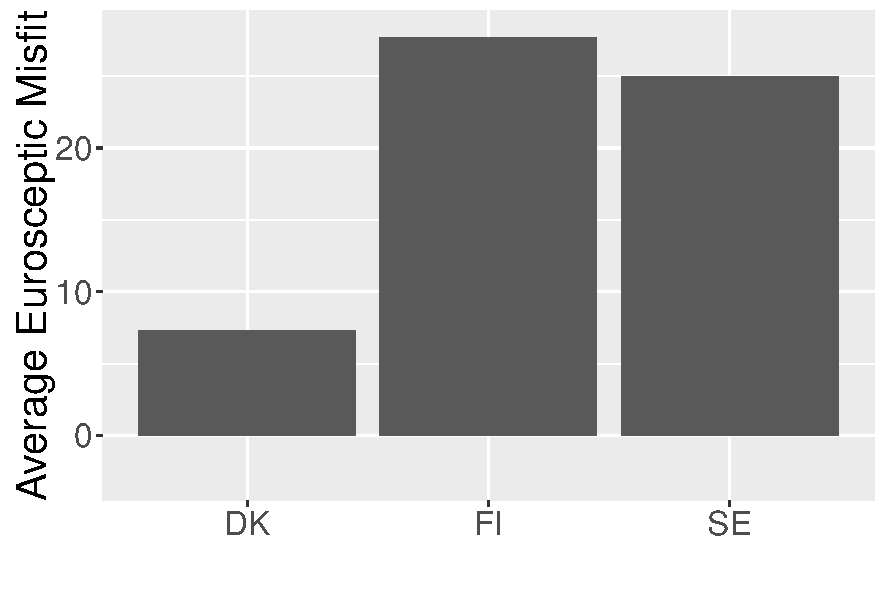
\includegraphics[width=65mm]{../../Analysis/Graphs/NE} & 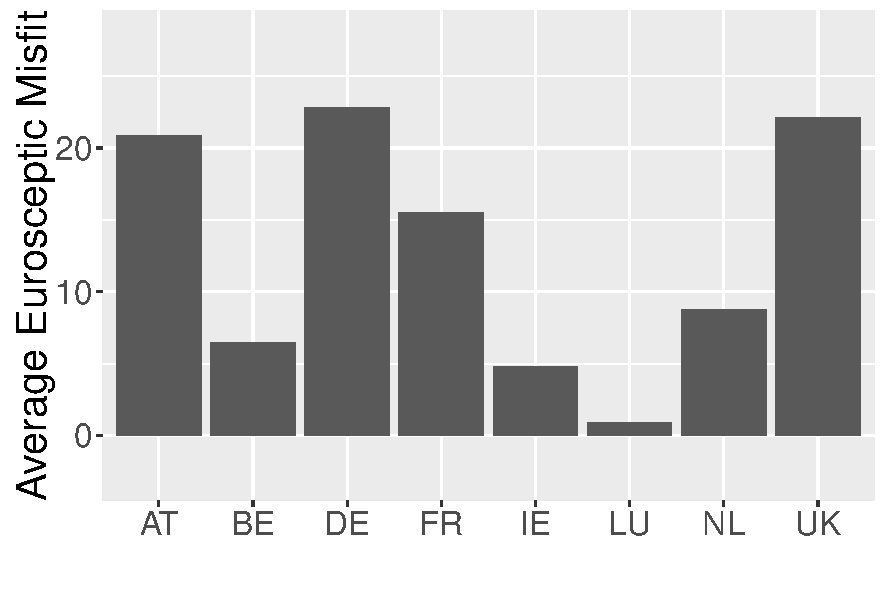
\includegraphics[width=65mm]{../../Analysis/Graphs/WE} \\
	(a) Northern Europe & (b) Western Europe \\[8pt]
	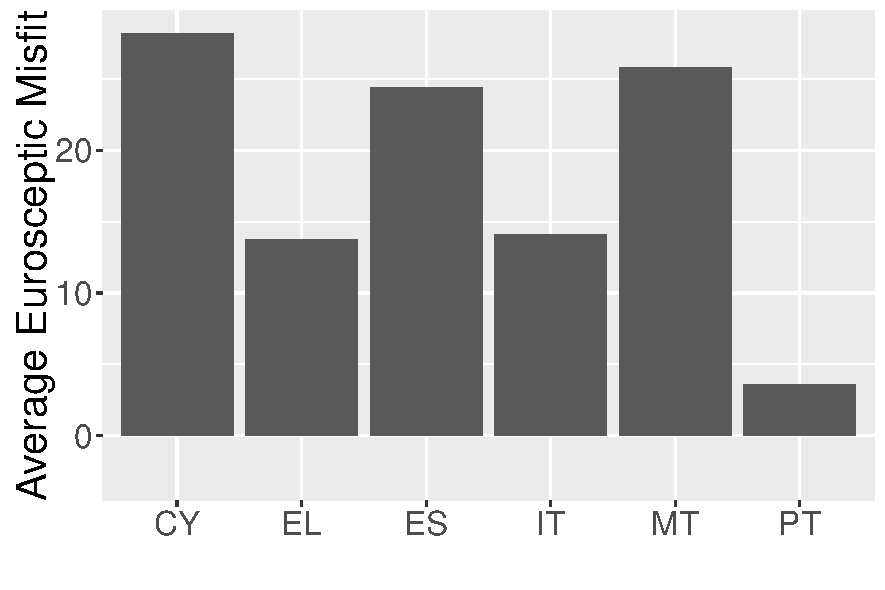
\includegraphics[width=65mm]{../../Analysis/Graphs/SE} & 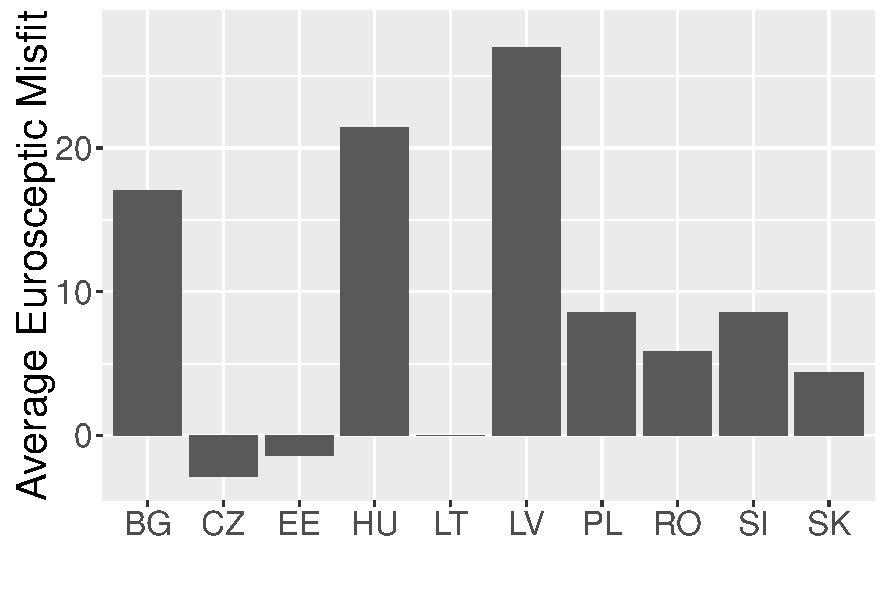
\includegraphics[width=65mm]{../../Analysis/Graphs/CEE} \\
	(c) Southern Europe & (d) Central/Eastern Europe \\[8pt]	
\end{tabular}
\caption*{Note: The y-axes are formatted uniformly across all graphs}	
\end{figure}

Trying to find regional patterns in the break up of the average Eurosceptic misfit across regions, as depicted by Figure~\ref{fig: Misfit Regions}, one is hard-pressed to find strong regional patterns. One noteworthy observation which can be drawn from sub-graph (d) is that there are a significant number of countries with negative Eurosceptic misfits in Central and Eastern Europe, paired with a slightly lower average overall. However, the size of the Eurosceptic misfit seems not to follow clear regional patterns aside from a better fit in Central and Eastern Europe, which had been observed before \cite{Taggart2002}.


\section{Post-regression analytics}
In order to choose the most appropriate model amongst the three models I outlined in Chapter 6.1, post-regression analytics were carried out to check for panel heteroskedasticity, cross-sectional dependence, serial correlation in the errors and the presence of unit roots in the data. 
To test the feasibility of the pooled OLS model, a Lagrange Multiplier Test for individual and or time effects on the pooled OLS model was conducted. It rejected, indicating that strong panel effects are present in the data, biasing OLS estimators. Therefore, I excluded the pooled OLS model from the discussion of the regression results below.
Testing for cross-sectional dependence failed, as both a Fries and Pesaran test applied to the data set returned errors. A Breusch-Pagan Lagrange-Multiplier test for cross-sectional dependence is unusable as the data had much larger N than T, which would have biased the results of the test \cite{Breusch1980}. Consequently, it is unclear whether there is cross-sectional correlation present in the data or not, which has to be considered in evaluating the results of estimations. 
In order to test for serial correlation in the error term, a Wooldridge test was conducted on the errors in the fixed-effects model \cite{Wooldridge2002}, as it is the most appropriate test given that the data set is short in \emph{T}. The test detects no serial correlation in the error terms.  
Finally, a Dickey-Fuller test for unit roots reveals that no unit root is present in the dependent variable, meaning that fixed-effects and random effects models are appropriate for the statistical analysis and first differencing of the data is not necessary. 
In the presence of strong panel effects, no serial correlation and unsure state of cross-sectional dependence, the pooled OLS model was discarded from the range of viable models. For the remaining two models, White heteroskedasticity-robust standard errors were calculated. I decided against using Panel Corrected Standard Errors (PCSE), as they tend to be heavily downward-biased unless \emph{T} is significantly larger than \emph{N} \cite{Beck1995}, which is not the case in my data set. The resulting estimates are found in Table ~\ref{tab: results}, where the column on the left (marked with a "1") shows the results from the fixed effects estimation and the column to the right of it shows the estimation results for the random effects model. 



% Table created by stargazer v.5.2 by Marek Hlavac, Harvard University. E-mail: hlavac at fas.harvard.edu
% Date and time: Mi, Mai 18, 2016 - 14:18:00
\begin{table}[!htbp] \centering 
  \caption{Fixed Effects and Random Effects Estimation with robust standard errors} 
  \label{tab: results} 
\begin{tabular}{@{\extracolsep{5pt}}lcc} 
\\[-1.8ex]\hline 
\hline \\[-1.8ex] 
 & \multicolumn{2}{c}{\textit{Dependent variable:}} \\ 
\cline{2-3} 
\\[-1.8ex] & \multicolumn{2}{c}{Eurosceptic Misfit} \\ 
 & FE & RE \\ 
\\[-1.8ex] & (1) & (2)\\ 
\hline \\[-1.8ex] 
 General Euroscepticism & 0.48$^{***}$ & 0.45$^{***}$ \\ 
  & (0.10) & (0.09) \\ 
  & & \\ 
 Instrumental Euroscepticism & 0.38$^{***}$ & 0.43$^{***}$ \\ 
  & (0.06) & (0.05) \\ 
  & & \\ 
 Polarisation Index & $-$1.52$^{*}$ & $-$1.92$^{**}$ \\ 
  & (0.84) & (0.74) \\ 
  & & \\ 
 Effective Number of Parties & 0.02 & $-$0.06 \\ 
  & (0.12) & (0.10) \\ 
  & & \\ 
 Membership Duration & 0.08 & 0.04 \\ 
  & (0.08) & (0.06) \\ 
  & & \\ 
 Central/Eastern European &  & $-$5.52$^{*}$ \\ 
  &  & (3.09) \\ 
  & & \\ 
 Constant &  & 0.57 \\ 
  &  & (3.47) \\ 
  & & \\ 
\hline \\[-1.8ex] 
\hline 
\hline \\[-1.8ex] 
\textit{Note:}  & \multicolumn{2}{r}{$^{*}$p$<$0.1; $^{**}$p$<$0.05; $^{***}$p$<$0.01} \\ 
\end{tabular} 
\end{table} 


\section{Inferential statistics}
After displaying descriptive statistics, the following subsections will present the results of the two statistical estimations. These aim to confirm or reject the four hypotheses which I put forward in the beginning of the paper.I will list them here again for convenience:
\begin{itemize}
	\item {\bf Hypothesis 1}: higher levels of popular Euroscepticism are associated with wider the Eurosceptic misfits
	\item {\bf Hypothesis 2}: higher levels of party system polarisation are associated with smaller Eurosceptic misfits
	\item {\bf Hypothesis 3}: the higher the number of effective parties in a party system, the smaller the Eurosceptic misfits
	\item {\bf Hypothesis 4}: the longer countries have been members of the EU, the wider their Eurosceptic misfits will be
	\item {\bf Hypothesis 5}: CEE Member States will have smaller Eurosceptic misfits than the remaining Member States on average
\end{itemize}

\subsection{Random effects model}
The results of the random effects model looks rather promising(labelled with a "RE" in Table ~\ref{tab: results}). The coefficient estimates on general Euroscepticism and instrumental Euroscepticism are highly statistically significant. 
Since both estimates are below, they indicate that rising levels of Euroscepticism in the population result in an increase of the Eurosceptic misfit. This could indicate that the translation of Eurosceptic sentiment into Eurosceptic votes is impeded by some national-level factors. These possibly prevent Eurosceptic parties from utilizing the Eurosceptic sentiments to garner votes. This is in line with my first hypothesis. Considering the ranges "general Euroscepticism" and "instrumental Euroscepticism" take on in the data set (compare Table~\ref{fig: summarystatistics}), the size of the coefficient estimate is also really substantively significant. 

According to the coefficient estimates, party system polarisation has a statistically significant negative effect on the Eurosceptic misfit. As I hypothesised above, the Eurosceptic misfit will be smaller in more polarised systems. The coefficient estimate of -1.92 is meaningful in terms of substantive significance, given that values for the polarisation index in the data set range from 0 to around 6.5. Hence, higher party system polarisation can significantly reduce the Eurosceptic misfit within a Member State. This lends support to my second hypothesis.

The effective number of parties, which measures fragmentation of the party system, does not seem to impact the Eurosceptic misfit at all, given the small size of the coefficient estimate and that its standard error far exceeds it in magnitude. This indicates that the estimation result is very unstable and even a tentative interpretation of the sign of the coefficient is unwise. This runs counter to my third hypothesis, as a higher number of effective parties does not seem to result in a smaller Eurosceptic misfit.

The coefficient estimate for membership duration is equally insignificant both statistically and substantively. This rejects my fourth hypothesis that longer membership durations are associated with wider Eurosceptic misfits.

In comparison, the dummy variable for location in Central and Eastern Europe is weakly statistically significant. Moreover, the size of the estimates is very substantive and indicates that the Eurosceptic misfit is significantly narrower in the CEE Member States. According to the estimates, the Eurosceptic misfit there is around 5.52 points lower on average. This finding lends tentative support to my fifth hypothesis that the Eurosceptic misfit is smaller in CEE Member States.

\subsection{Fixed effects model}
General Euroscepticism , which shows the percentage of respondents who said that their country's membership of the EC/EU is a bad thing, has a positive effect on the Eurosceptic misfit. This means that as the percentage of generally Eurosceptic voters within member states increased, the Eurosceptic gap within these countries grew with it. For each percentage point increase in the national generally Eurosceptic public, the Eurosceptic misfit within the respective country widened by 0.48 points on average. This result is highly statistically significant.
The coefficient estimate for the instrumental Euroscepticism variable is also positive and highly statistically significant. As the share of Eurosceptic respondents within a country increases by one unit, the Eurosceptic misfit within that same country increases by 0.38 points.
These two findings support my first hypothesis. As with the estimates of the random effects model, they indicate that Eurosceptic votes lag behind rises in popular Eurosceptic sentiment.

Party system polarisation has a negative effect on the size of the Eurosceptic misfit, indicating that as the party system within a country becomes more polarized, the Eurosceptic misfit in that country shrinks. This result is weakly statistically significant. The size of the coefficient estimate is not too dissimilar from the random effects model, so it is substantively significant also. This lends support to Hypothesis 2 that party system polarisation shrinks the Eurosceptic misfit.

The coefficient estimate on the effective number of parties is very insignificant both on statistical and substantive terms. Contrary to what I expected, an increase in the number of effective parties does not result in a a smaller Eurosceptic misfit. Also, the mathematical sign of the coefficient is positive. This is surprising as I would have expected an increase in party system fragmentation to be accompanied by a smaller Eurosceptic misfit, which would have meant a negative coefficient on the effective number of parties. It is important to remember that this estimate is not statistically different from 0. Given that the standard error exceeds the size of the coefficient, it is plausible that the effect could be also negative but fails to register as a significant effect due to the small sample size of the study or insufficient variation in the number of parties within member states across time. Overall, this finding rejects my third hypothesis that an increase in the number of effective parties is associated with a smaller Eurosceptic misfit.

As with the random effects model, the coefficient estimate for the variable measuring membership duration is not statistically nor substantively significant. As with the random effects model, this runs counter to my fourth hypothesis. 

Because fixed effects model only estimates coefficient for time-varying variables, it does not allow me to assess the effect of being among the CEE Member States, so no judgement can be passed on Hypothesis 5.

The fixed effects estimation allows me to report the amount of unobserved time-invariant variation in the Eurosceptic misfit specific to each country which is removed through demeaning of the data. They are mapped in Figure ~\ref{fig: country-specific_error} and can be interpreted similar to intercepts. They show that a lot of time-constant variation in the Eurosceptic misfit exists between Member States which cannot be explained by my model. It can be interpreted as the base Eurosceptic misfit which pre-exists within the Member States. Figure ~\ref{fig: country-specific_error} shows that these misfits vary widely between countries. No clear pattern is discernible between year of accession or geographic location and the size of the country-specific error. This indicates that a lot of the variation in the Eurosceptic misfit is due to uniquely national factors, which lie deeper within the national party system, out of reach of the variables employed in my model. They possibly relate to the way in which the competitive space of the party system is structured and how parties position themselves within it. 

\begin{landscape}
	\begin{figure}
		\centering
		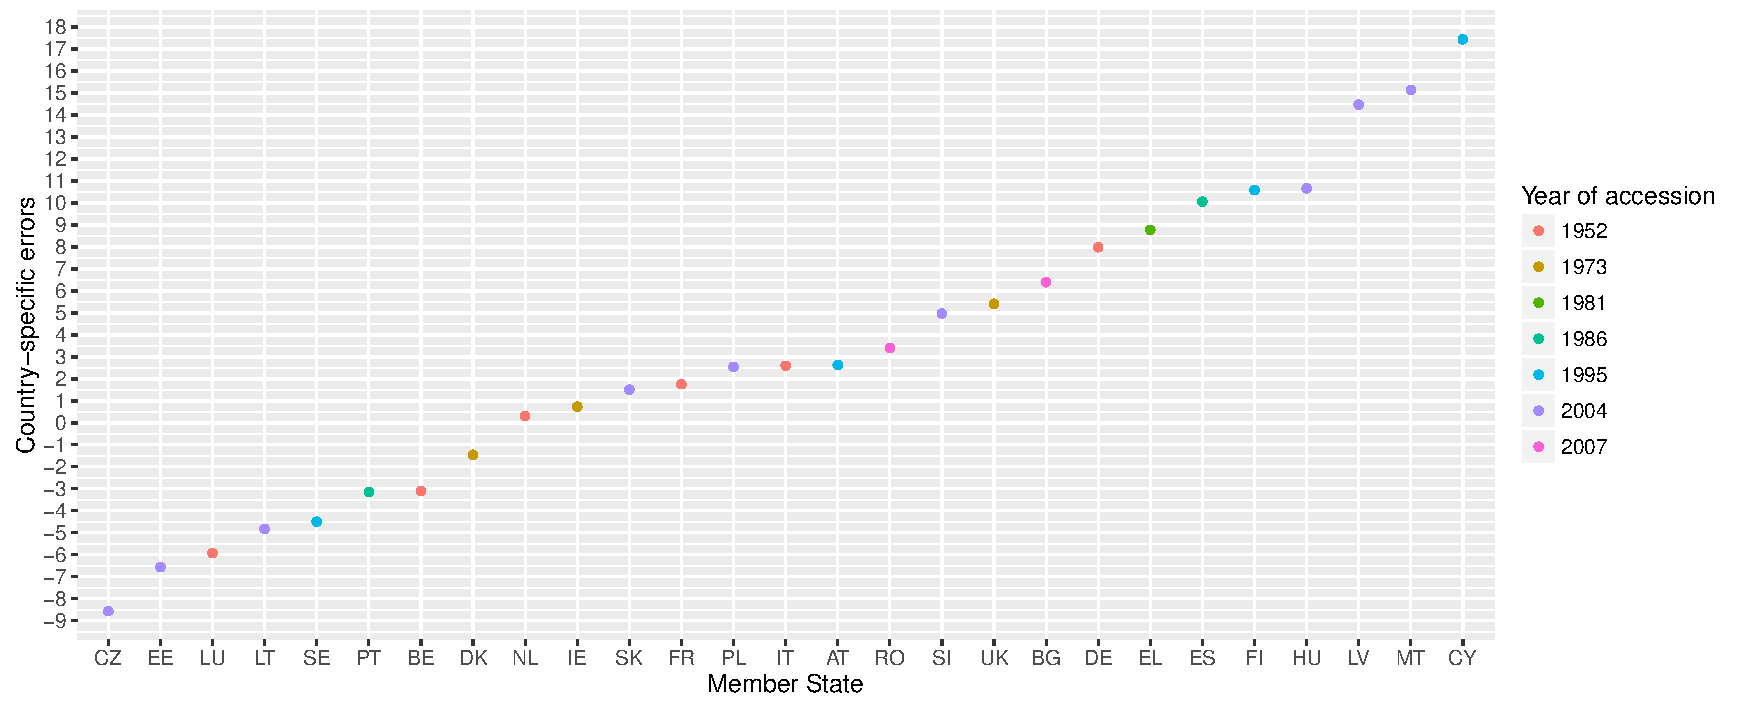
\includegraphics[width=1.2\linewidth]{../../Analysis/Graphs/country-specific_error}
		\caption{Idiosyncratic Error by Member State}
		\label{fig: country-specific_error}
	\end{figure}
\end{landscape}

\subsection{Comparing random effects and fixed effects models}
Comparing the results of the different estimation methods side by side, the random effects model seems a lot more promising, as its higher efficiency allows me to find stronger and more nuanced effects in the data. Upon visual inspection, the models do not look very consistent. Some point estimates are decently similar, others differ quite significantly. A Hausman test comparing the two models for inconsistencies does not find the random effects model to be significantly inconsistent in comparison, which suggests that the random effects estimate is reliable. However, since the data under scrutiny is country-level macro data, a crucial assumption underpinning the random effects estimator is violated, as the observations are not part of a random sample which is drawn from a larger population. This makes the results  from the random effects estimation unreliable and forces me to rely on the more consistent fixed effects estimator \cite{Wooldridge2003}. Given this limitation, I can argue that a Eurosceptic misfit exists and that there is some indication that it is modulated by the polarisation within party systems, but the evidence does not support the inference of causality. Furthermore, there is evidence that  general Euroscepticism and Instrumental Euroscepticism generally lag behind the vote shares obtained by Eurosceptic parties. However given the limited number of variables in the data set and the complex nature of national party systems, these relationships come with big caveats as they could be caused by lurking time-variant variables which were not controlled for in the model. 

\chapter{Conclusion}
The Eurosceptic misfit exists in most countries of the EU persistently across all the time periods studied. On an aggregate EU-level it has remained relatively stable ever since the 1994 EP elections. Looking at the development of the Eurosceptic misfit in the initial EU-6 results in a much more chaotic picture. Different countries exhibit highly differing patterns in the evolution of the Eurosceptic misfit over the years. Stark fluctuations in the misfit can be observed between election cycles, especially in France and Luxembourg.  The volatility of the misfit suggests that it is shaped by dynamics which experience stark changes in between election rounds. These could be related to the structuring of party competition within the party system, electoral campaigns or hot-button issues which readily sway voters.This means that future models trying to comprehensively model the Eurosceptic misfit would need variables capturing this volatility. Hence, future models should add such variables to the ones measuring relatively stable properties of party systems, such as polarisation and fragmentation.

In my research question I asked which national-level properties affect the Eurosceptic misfit. Summarising the statistical analysis, the following conclusions can be drawn: 

The descriptive statistics and visualisation indicate that CEE Member States might exhibit smaller Eurosceptic misfits compared to the remaining Member States, but no other regional patters seem to exist. This hypothesis also finds support in the random effects model, which should be taken with a grain of salt, however.

The inferential statistics reveal higher levels of both general and instrumental Euroscepticism in the public are associated with bigger Eurosceptic misfits. The coefficient estimates of generally Eurosceptic attitudes and instrumentally Eurosceptic attitudes are highly substantively and statistically significant. The effect is found in both the random effects and the fixed effects model and can be accepted as relatively solid.Maybe this is the result of a sluggish translation of Eurosceptic attitudes into Eurosceptic votes, maybe some mediating variable prevents Eurosceptic parties from "cashing in" on the popular attitudes against integration. 

The statistical estimation also shows consistently that higher levels of party system polarisation lead to smaller Eurosceptic misfits. As this finding is supported in both statistical models, it can be be accepted with a reasonable degree of certainty.

Both the effective number of parties and EU-membership duration are shown to not have any significant effect on the size of the Eurosceptic misfit, contrary to the hypotheses made at the beginning of the paper.  

The fact that country-specific errors shown in Figure~\ref{fig: country-specific_error} suggests that there is large variation in the size of the Europsceptic misfit which is not explained by my statistical model. The Eurosceptic misfit might be driven by an interplay of more complex variables on the national level. Moreover, this thesis limited itself to examining macro-level variables' effect on aggregated data. Thus, it does not allow me to directly observe the Eurosceptic misfit on the individual level: people who hold Eurosceptic attitudes but who choose not to vote for a Eurosceptic party. Further research employing a multi-level hierarchical model which looks at individuals embedded into their national party systems could help unravelling causal effects more closely.

As for possible factors preventing the "translation" of Eurosceptic attitudes into votes on the national level, several mechanisms seem plausible. Perhaps the outsider status of parties outside of the political mainstream is decisive. This causes voters to not see Eurosceptic parties as serious contenders, incompetent of wielding political power. Possibly, an upper ceiling of protest-driven Eurosceptic vote exists; protest voters support Eurosceptic parties to send a message to mainstream parties, but they do not \emph{really} want Eurosceptic parties to govern themselves. Another possible confounding factor could be the timing of the EP election in relation to the last national election.
At this point, all of these musings remain speculation that cannot be answered given the data at hand, but which could open up avenues for further research.


\pagebreak

% R package citations
\nocite{R-car}
\nocite{R-dplyr}
\nocite{R-ggplot2}
\nocite{R-haven}
\nocite{R-knitr}
\nocite{R-lmtest}
\nocite{R-plm}
\nocite{R-stargazer}

\bibliographystyle{apacite}
\bibliography{bibliography}


\pagebreak



{\LARGE Statement of Authorship}



I hereby confirm and certify that this master thesis is my own work. All ideas and language of others are acknowledged in the text. All references and verbatim extracts are properly quoted and all other sources of information are specifically and clearly designated. 



DATE:




NAME:




SIGNATURE:

\end{document}
